\documentclass[conference]{IEEEtran}

\usepackage[utf8]{inputenc}
\usepackage[T1]{fontenc}
\usepackage[spanish,es-nodecimaldot,es-noshorthands]{babel}
\usepackage{amsmath,amssymb}
\usepackage{graphicx}
\usepackage{booktabs}
\usepackage{array}
\usepackage{xcolor}
\usepackage{url}
\usepackage{cite}
\usepackage{tikz}
\usetikzlibrary{positioning,arrows.meta,calc}

\graphicspath{{figuras/}}

% Marca de datos por completar (quitar cuando se llenen)
\newcommand{\pend}[1]{\textcolor{red}{[#1]}}

\begin{document}

\title{VALIDACIÓN EXPERIMENTAL DE LA CURVA BER VS. $E_b/N_0$ DE UN ENLACE BFSK PARA TELEMETRÍA INDUSTRIAL CON USRP 2920 Y HACKRF ONE}

\author{
\IEEEauthorblockN{Edward Andres Pacheco Jurado- 2222236, Angely Yulitza Vásquez Lozada- 2222240\\
Daniel Eduardo Suarez Jaimes- 2222228}
\IEEEauthorblockA{Universidad Industrial de Santander\\
Escuela de Ingenierías Eléctrica, Electrónica y de Telecomunicaciones\\
GitHub: \url{https://github.com/EDWARDPJ26/2026_2_CommII_A1_GA1D_PRoYECTO_FINAL}}
}

\maketitle

\begin{abstract}
This work presents the final experimental validation of the binary frequency shift keying (BFSK) link designed for an industrial telemetry application. The common BER instrumentation module was integrated into a copy of the working receiver: controlled AWGN was added after the rate adaptation of the HackRF One samples (1~MS/s) and the bit error rate was measured over an automatic $E_b/N_0$ sweep, while an NI USRP 2920 transmitted a fixed telemetry frame (preamble, SFD and a 61-character ASCII payload) at 870~MHz over the air. The measurement revealed a poor initial receiver performance, which was corrected by narrowing the channel filter to 35~kHz, using an integrate-and-dump filter and replacing the manual sampling delay by a Gardner symbol synchronizer. Because transmitter and receiver run on different computers, the known reference sequence was aligned automatically by correlation. In clean conditions the BER was zero, and the measured curves reach $\text{BER} = 10^{-3}$ at 14.3~dB (ASCII payload) and 14.2~dB (PN9-whitened payload), about 0.5~dB from the simulated reference, well within the 2~dB acceptance criterion.
\end{abstract}

\begin{IEEEkeywords}
BFSK, BER, $E_b/N_0$, SDR, USRP 2920, HackRF One, GNU Radio, sincronización de símbolo, telemetría industrial.
\end{IEEEkeywords}

\section{Introducción}

En las fases anteriores el enlace BFSK para telemetría industrial se diseñó y verificó en simulación~\cite{guia1,guia2} y después se llevó a un enlace físico por aire con un USRP 2920 como transmisor y un HackRF One como receptor~\cite{guia3}. En esa etapa se comprobó que el receptor recuperaba la secuencia transmitida, pero no se cuantificó su desempeño.

Esta fase cierra el proyecto con una medición objetiva: la curva de tasa de error de bit (BER) frente a $E_b/N_0$ del sistema real. Para ello se integró al flujograma del grupo el módulo común de instrumentación entregado por el curso~\cite{guia4,guia4a}, que añade ruido blanco gaussiano controlado a la señal recibida, recorre automáticamente los niveles de $E_b/N_0$ y compara los bits recibidos con una referencia conocida. La curva medida se compara con la obtenida en simulación con el mismo receptor; el criterio de conformidad es una penalización de a lo sumo 2~dB en $\text{BER} = 10^{-3}$.

\section{Metodología}

\subsection{Montaje y parámetros del sistema}

El enlace se mantuvo como en la Fase~3: el transmisor se ejecuta en el PC conectado por Ethernet al USRP 2920 y el receptor en un portátil con el HackRF One por USB; ambos usan antenas del laboratorio y la señal viaja por aire, porque no se dispuso de cable coaxial ni atenuadores. El Cuadro~\ref{tab:param} resume los valores reales del sistema que se vincularon con la instrumentación.

\begin{table}[!t]
\centering
\caption{Parámetros reales del sistema usados en la medición.}
\label{tab:param}
\begin{tabular}{>{\raggedright}p{2.6cm}>{\raggedright}p{1.6cm}p{3.4cm}}
\toprule
Parámetro & Valor & Observación \\
\midrule
Modulación & 2FSK (BFSK) & Detección no coherente con discriminador. \\
Bits por símbolo & $\log_2 M = 1$ & En BFSK símbolo y bit coinciden. \\
$R_s$ & 10~kbaud & Igual que en las fases 2 y 3. \\
$R_b = R_s \cdot \log_2 M$ & 10~kb/s & \\
$bb\_rate$ & 1~MS/s & Tasa I/Q a la entrada de \texttt{e\_EbN0\_Sweep}. \\
$sps$ & 100 & $bb\_rate/R_s$. \\
$\Delta f$, $h$ & 20~kHz, 4 & Tonos en $f_c \pm 20$~kHz. \\
Ancho de banda & 60~kHz & Regla de Carson: $2(\Delta f + R_s)$. \\
Amplitud de referencia & 1 & Envolvente constante del modulador; se escala con \texttt{tx\_amp} = 0.7 antes del DAC. \\
$f_c$ & 870~MHz & \\
Ganancia TX (USRP) & $\approx 30$~dB & Ajustada en la GUI durante la medición. \\
Tasa del HackRF & 4~MS/s & Decimación por 4 hasta $bb\_rate$. \\
LNA / VGA / AMP & 16 / 20 / 0~dB & Valores por defecto del receptor. \\
\bottomrule
\end{tabular}
\end{table}

\subsection{Secuencia de prueba}

Como el transmisor y el receptor están en computadores distintos, la BER solo puede medirse si ambos conocen la misma secuencia~\cite{guia4a}. Se definió una trama fija de telemetría inspirada en IEEE 802.15.4g (SUN-FSK)~\cite{ieee154g}, que se transmite en bucle:
\begin{itemize}
\item preámbulo \texttt{0x55555555} (32~bits) y palabra de sincronización (SFD) \texttt{0x904E} (16~bits);
\item carga útil ASCII de 61 caracteres con lecturas simuladas fijas de un sensor de planta: \texttt{ID:S01;T:24.5C;HR:15\%;ALT:2500msnm;} \texttt{P:184kPa;NIV:72\%;Q:3.4m3/h}.
\end{itemize}
La trama tiene 536~bits y dura 53.6~ms. Se midieron dos variantes, seleccionadas con la variable \texttt{pn9}, que debe valer lo mismo en el Tx y en el Rx:
\begin{itemize}
\item \texttt{pn9 = 0}: carga en ASCII sin blanqueo. La proporción de unos es 0.451.
\item \texttt{pn9 = 1}: carga blanqueada con la secuencia PN9 ($x^9 + x^5 + 1$, semilla \texttt{0x1FF}), como hace 802.15.4g. La proporción de unos sube a 0.498. El preámbulo y el SFD nunca se blanquean.
\end{itemize}
El mismo módulo de Python (\texttt{trama\_telemetria}) genera la trama en los dos flujogramas, de modo que la referencia es idéntica en ambos extremos.

\subsection{Transmisor}

La Fig.~\ref{fig:flujotx} muestra el transmisor de la Fase~4. Es el transmisor limpio de las fases anteriores con la trama de telemetría en lugar del patrón de 16~bits: Vector Source en bucle, mapeo NRZ ($0 \rightarrow -1$, $1 \rightarrow +1$), Repeat por $sps = 100$, Frequency Mod con sensibilidad $2\pi\Delta f/f_s = 0.1257$~rad/muestra, Multiply Const (\texttt{tx\_amp} = 0.7) y UHD: USRP Sink a 1~MS/s con Sync = \texttt{none}. El transmisor no inyecta ruido: todo el AWGN de la medición lo añade el instrumento en el receptor.

\begin{figure*}[!t]
\centering
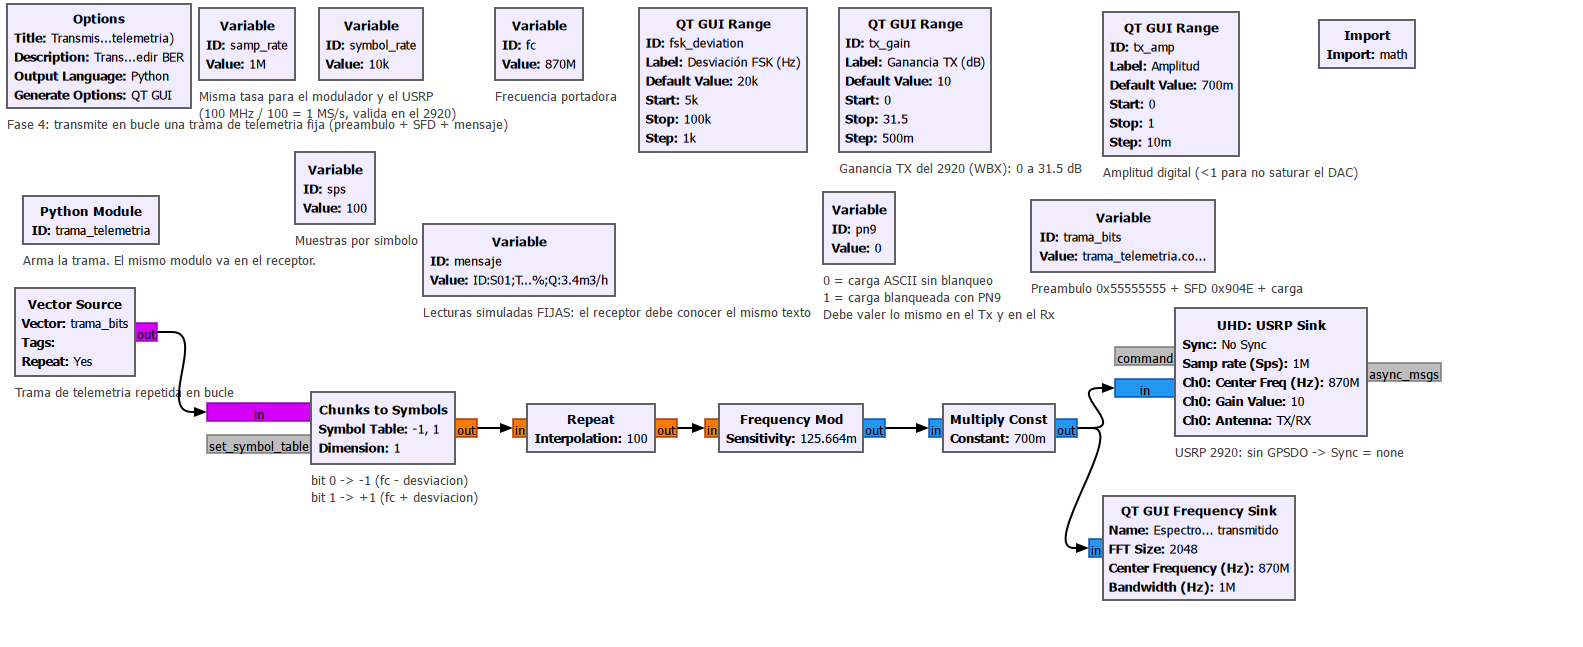
\includegraphics[width=\textwidth]{flujo_tx.png}
\caption{Flujograma del transmisor \texttt{Transmisor\_FSK\_USRP\_Fase4.grc}. La trama de telemetría (preámbulo + SFD + carga) se repite en bucle; \texttt{pn9} selecciona la carga ASCII o blanqueada. La ganancia del USRP se ajustó en la GUI a unos 30~dB durante la medición.}
\label{fig:flujotx}
\end{figure*}

\subsection{Integración de la instrumentación en el receptor}

Siguiendo la guía, la instrumentación se integró en una \textbf{copia} del receptor funcional (\texttt{Receptor\_FSK\_HackRF\_Fase4\_v2.grc}); el receptor de la Fase~3 se conservó sin cambios. Las Figs.~\ref{fig:flujorx1} y~\ref{fig:flujorx2} muestran el flujograma, dividido en dos partes por su tamaño. La cadena de medición es
\begin{center}
\small osmocom Source $\rightarrow$ adaptación de tasa $\rightarrow$ \texttt{e\_EbN0\_Sweep} $\rightarrow$ receptor digital,\\
bits Tx (referencia) + bits Rx $\rightarrow$ \texttt{e\_BER\_Curve} $\rightarrow$ Vector Sink y CSV.
\end{center}

\begin{figure*}[!t]
\centering
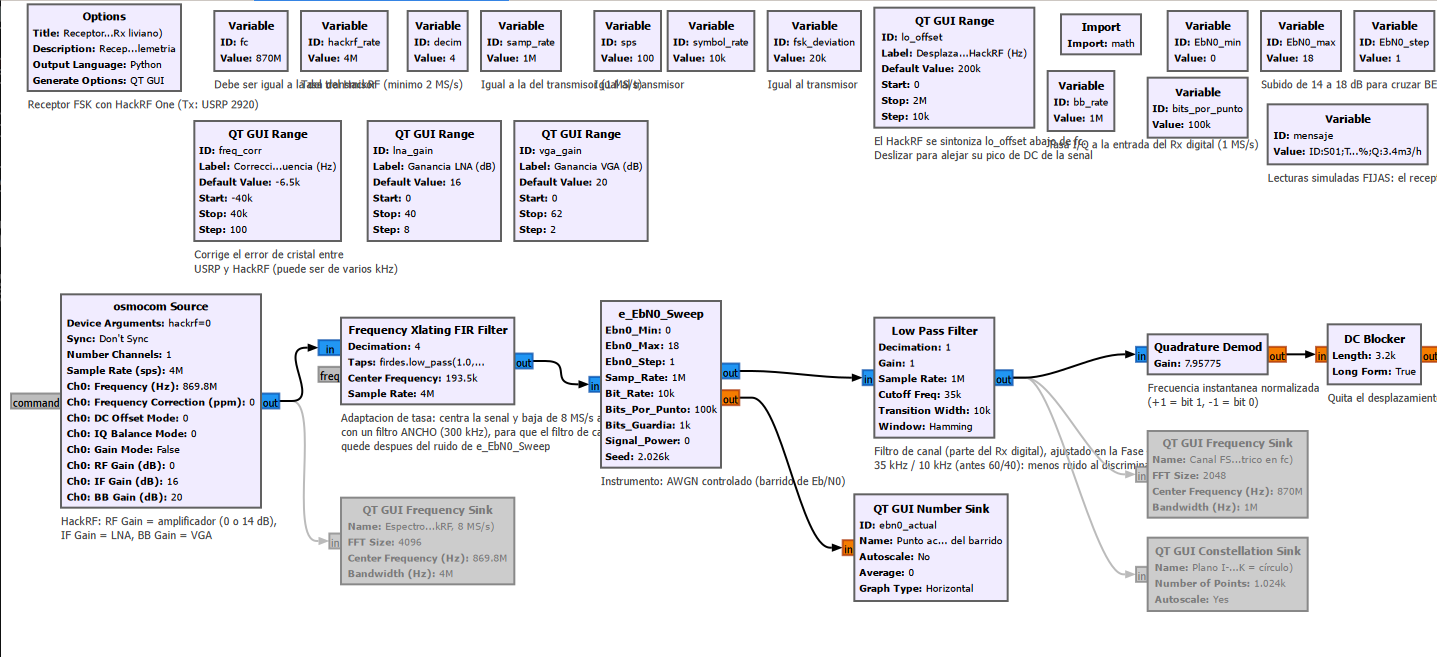
\includegraphics[width=\textwidth]{flujo_rx1.png}
\caption{Flujograma del receptor \texttt{Receptor\_FSK\_HackRF\_Fase4\_v2.grc}, parte 1: osmocom Source (4~MS/s, sintonizado en $f_c - \texttt{lo\_offset}$), Frequency Xlating FIR Filter (adaptación de tasa con decimación por 4), \texttt{e\_EbN0\_Sweep}, filtro de canal de 35~kHz, Quadrature Demod y DC Blocker. Los bloques en gris son gráficas deshabilitadas para aligerar el receptor.}
\label{fig:flujorx1}
\end{figure*}

\begin{figure*}[!t]
\centering
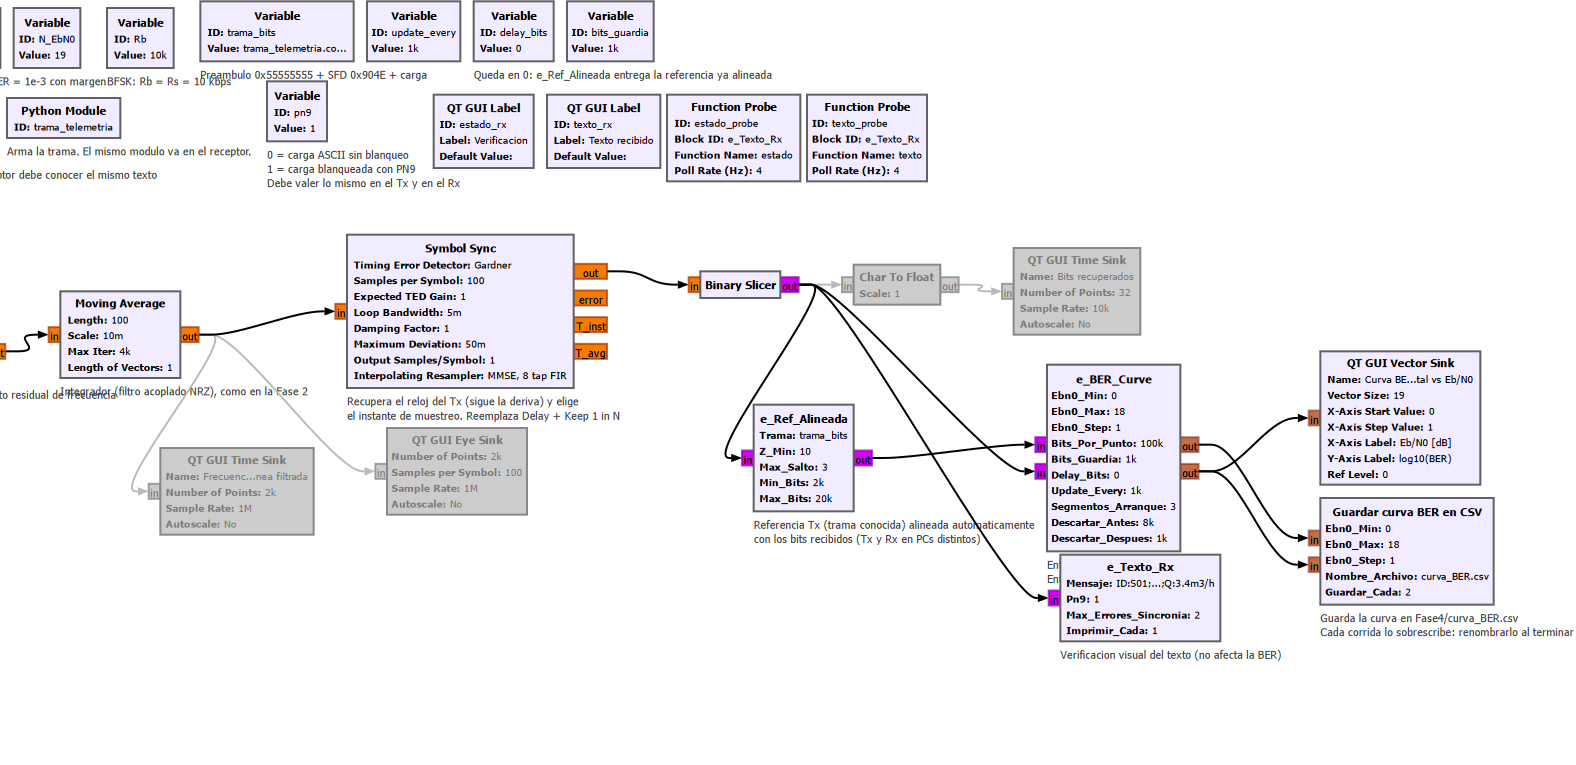
\includegraphics[width=\textwidth]{flujo_rx2.png}
\caption{Flujograma del receptor, parte 2: integrador (Moving Average), Symbol Sync (Gardner), Binary Slicer, referencia alineada \texttt{e\_Ref\_Alineada}, \texttt{e\_BER\_Curve} con su QT GUI Vector Sink y el bloque que guarda \texttt{curva\_BER.csv}, además de la verificación del texto (\texttt{e\_Texto\_Rx}).}
\label{fig:flujorx2}
\end{figure*}

El punto de inserción del ruido es importante. En el receptor de la Fase~3 un único Xlating FIR hacía a la vez la traslación, la decimación y el filtrado de canal. Se separó en dos etapas: primero un Xlating FIR con un filtro \emph{ancho} (300~kHz de corte) que solo recentra la señal ($\texttt{lo\_offset} + \texttt{freq\_corr}$) y baja la tasa a $bb\_rate = 1$~MS/s; después \texttt{e\_EbN0\_Sweep}; y después el filtro de canal. Así el ruido añadido pasa por el filtro de canal como lo haría el ruido térmico de un receptor real, y el instrumento trabaja a la tasa I/Q correcta. En el hardware no hay ningún bloque Throttle: el ritmo lo impone el ADC del HackRF.

El Cuadro~\ref{tab:barrido} recoge los valores del instrumento. \texttt{e\_EbN0\_Sweep} mide la potencia media $P_s$ de la señal recibida antes de añadir el ruido y calcula la potencia del ruido complejo como
\begin{equation}
P_n = \frac{P_s \, f_s}{R_b \cdot 10^{(E_b/N_0)/10}},
\label{eq:pn}
\end{equation}
con $f_s = bb\_rate$. Cada punto se mantiene durante \texttt{bits\_guardia} + \texttt{bits\_por\_punto} bits, y \texttt{e\_BER\_Curve} descarta los bits de guardia para que el receptor se estabilice tras cada cambio de nivel.

\begin{table}[!t]
\centering
\caption{Parámetros del barrido BER.}
\label{tab:barrido}
\begin{tabular}{>{\raggedright}p{2.3cm}>{\raggedright}p{1.4cm}p{3.9cm}}
\toprule
Variable & Valor & Comentario \\
\midrule
\texttt{Rb} & 10~kb/s & BFSK: $R_b = R_s$. \\
\texttt{bb\_rate} & 1~MS/s & Después de la decimación por 4. \\
\texttt{EbN0\_min}, \texttt{EbN0\_step} & 0~dB, 1~dB & Valores comunes. \\
\texttt{EbN0\_max} & 18~dB & Se extendió de 14 a 18~dB (ver texto). \\
\texttt{N\_EbN0} & 19 & Resultado del rango 0--18~dB. \\
\texttt{bits\_por\_punto} & 100\,000 & Valor común. \\
\texttt{bits\_guardia} & 1000 & Valor común. \\
\texttt{delay\_bits} & 0 & La referencia llega ya alineada (Sec.~\ref{sec:alineacion}). \\
\texttt{update\_every} & 1000 & Valor común. \\
\bottomrule
\end{tabular}
\end{table}

El rango común de la guía es de 0 a 14~dB. Con este receptor la BER en 14~dB todavía es del orden de $10^{-3}$, así que el barrido se extendió hasta 18~dB para observar toda la caída de la curva por debajo del punto de comparación. Los puntos de 0 a 14~dB, con el mismo paso de 1~dB, siguen disponibles y son los comparables con los demás grupos.

\subsection{Ajuste del receptor}

Antes de llevar la medición al laboratorio, la cadena completa se probó con un banco de pruebas en Python sin hardware: transmisor, conversión a 8~MS/s, desplazamiento por \texttt{lo\_offset} y deriva de reloj de 20~ppm entre radios. La medición con el receptor de la Fase~3 reveló un desempeño pobre (Cuadro~\ref{tab:ajuste}), con dos causas:
\begin{itemize}
\item el filtro de canal de 60/40~kHz dejaba pasar demasiado ruido al discriminador, que entraba en la zona de efecto umbral;
\item el muestreo con \texttt{Delay} + \texttt{Keep 1 in N} es fijo: el retardo por defecto caía cerca del peor instante y, con la deriva de reloj entre radios, el instante óptimo se desplaza un símbolo cada pocos segundos.
\end{itemize}

\begin{table}[!t]
\centering
\caption{Ajuste del receptor (banco de pruebas, simulación).}
\label{tab:ajuste}
\begin{tabular}{>{\raggedright}p{4.4cm}cc}
\toprule
Receptor & BER @ 12~dB & BER @ 14~dB \\
\midrule
Fase 3 (Delay + Keep 1 in N, LPF, filtro 60/40~kHz) & $1.3\times10^{-1}$ & $5.7\times10^{-2}$ \\
Symbol Sync + LPF + filtro 40/20~kHz & $1.6\times10^{-2}$ & $2.6\times10^{-3}$ \\
Symbol Sync + integrador + filtro 40/20~kHz & $1.1\times10^{-2}$ & $1.1\times10^{-3}$ \\
\textbf{Symbol Sync + integrador + filtro 35/10~kHz} & $\mathbf{7.6\times10^{-3}}$ & $\mathbf{7.6\times10^{-4}}$ \\
\bottomrule
\end{tabular}
\end{table}

La configuración final del receptor digital es:
\begin{itemize}
\item \textbf{Filtro de canal}: pasa bajas a 1~MS/s con corte en 35~kHz ($\Delta f + 1.5 R_s$) y transición de 10~kHz, el mismo que se diseñó en la Fase~2.
\item \textbf{Integrador}: Moving Average de longitud $sps$ y escala $1/sps$, que es el filtro acoplado para pulsos NRZ, en lugar del pasa bajas de 10~kHz.
\item \textbf{Symbol Sync}: detector de error de Gardner, $sps = 100$, ancho de banda de lazo 0.005, amortiguamiento 1, desviación máxima 0.05 e interpolador MMSE de 8 taps~\cite{symsync}. Sustituye a \texttt{Delay} + \texttt{Keep 1 in N} y sigue la deriva de reloj. Con desviación máxima de 1.5, o con anchos de lazo de 0.02 o 0.002, el lazo se deslizaba en presencia de ruido.
\end{itemize}
Estos cambios son de ajuste del receptor: corrigen un desempeño deficiente que la propia medición puso en evidencia, y no modifican ningún parámetro de diseño del enlace ($R_s$, $\Delta f$, $sps$, $f_c$).

En el laboratorio se ajustaron además los parámetros propios del hardware. Con $\texttt{lo\_offset} = 0$, el pico de DC y el desbalance I/Q del HackRF caían dentro del canal y el plano I-Q salía elíptico (Fig.~\ref{fig:iq}a); con $\texttt{lo\_offset} = 200$~kHz el anillo es circular (Fig.~\ref{fig:iq}b). El error de frecuencia entre los cristales del USRP y del HackRF se corrigió con $\texttt{freq\_corr} = -6.5$~kHz, hasta que los dos lóbulos de la FSK quedaron simétricos en el canal centrado (Fig.~\ref{fig:limpiagui}).

\subsection{Alineación de Tx y Rx: \texttt{delay\_bits} y \texttt{delay\_symbols}}
\label{sec:alineacion}

La guía propone ajustar \texttt{delay\_bits} a mano hasta obtener $\text{BER} \approx 0$ en condición limpia. En este enlace ese procedimiento no es estable, por dos razones:
\begin{itemize}
\item el Tx y el Rx corren en computadores distintos y arrancan en instantes arbitrarios, así que el desfase entre la trama transmitida y la recibida cambia en cada ejecución;
\item cuando el portátil del receptor pierde muestras (overflows del HackRF, ``O'' en consola, Fig.~\ref{fig:consola}), el flujo de bits salta una cantidad arbitraria de bits y cualquier retardo fijo queda desalineado.
\end{itemize}
Por eso se sustituyó el Vector Source de referencia por un bloque propio, \texttt{e\_Ref\_Alineada}, que genera la trama conocida \emph{ya alineada} con los bits recibidos. El bloque calcula la correlación circular entre los últimos bits recibidos y la trama de 536~bits, y fija el desfase cuando el pico supera $z \geq 10$ desviaciones estándar. En la Fig.~\ref{fig:consola} se ve la alineación al arrancar: desfase de 49~bits con $z = 10.4$ tras 830~bits, dentro de los 1000~bits de guardia. Después corrige deslizamientos de $\pm 3$~bits y, si detecta un salto mayor, se realinea globalmente y emite una etiqueta \texttt{realineo}; \texttt{e\_BER\_Curve} descarta los 8000~bits anteriores y los 1000 posteriores a cada realineo para no contar como errores del canal los bits comparados con la referencia desalineada. Con la referencia alineada, \texttt{delay\_bits} = 0.

La validación sin hardware confirmó que el método no sesga la medida: sin errores reales da $\text{BER} = 0$, y con errores reales del 1, 10, 25 y 35~\% devuelve la BER correcta. En el laboratorio hubo cuatro realineos por medición, con el 1.2~\% (ASCII) y el 1.9~\% (PN9) de los bits descartados.

En BFSK cada símbolo transporta un bit, de modo que los símbolos Tx y Rx coinciden con los bits y \texttt{delay\_symbols} es igual a \texttt{delay\_bits}; la SER es igual a la BER y no se analiza por separado~\cite{guia4a}.

\subsection{Procedimiento de medición}

\begin{enumerate}
\item Se ejecutó primero el transmisor y después el receptor, porque \texttt{e\_EbN0\_Sweep} promedia la potencia de la señal desde que arranca.
\item Con el barrido detenido se ajustaron \texttt{lo\_offset}, \texttt{freq\_corr} y las ganancias, verificando que el texto llegara completo, y se guardaron como valores por defecto del flujograma, porque al reiniciar los controles vuelven a ese valor.
\item \textbf{Condición limpia}: barrido de 30 a 48~dB (19 puntos) con 10\,000~bits por punto. A esos niveles el ruido añadido es despreciable y debe obtenerse $\text{BER} \approx 0$.
\item \textbf{Medición}: barrido de 0 a 18~dB con 100\,000~bits por punto, dejando correr varias pasadas sin mover las antenas ni usar el portátil. Al terminar, el archivo \texttt{curva\_BER.csv} se copió sin editar como \texttt{curva\_BER\_ascii.csv}.
\item Se repitió con \texttt{pn9 = 1} en los dos extremos (\texttt{curva\_BER\_pn9.csv}).
\end{enumerate}

\section{Resultados}

\subsection{Condición limpia}

La Fig.~\ref{fig:limpia} muestra el barrido de 30 a 48~dB: los 19 puntos tienen $\text{BER} = 0$. Como la escala es logarítmica, los puntos sin errores se dibujan en la cota $3/N$ (regla del tres, intervalo de confianza del 95~\%), que con los bits contados por punto es del orden de $10^{-4}$. En la misma condición, la verificación de texto acumuló 3370 tramas correctas de 3375 recibidas (Fig.~\ref{fig:limpiagui}); las tramas con error corresponden al arranque, antes de la alineación. Esto confirma que la referencia está bien alineada y que, sin ruido añadido, el enlace por aire no introduce errores.

\begin{figure}[!t]
\centering
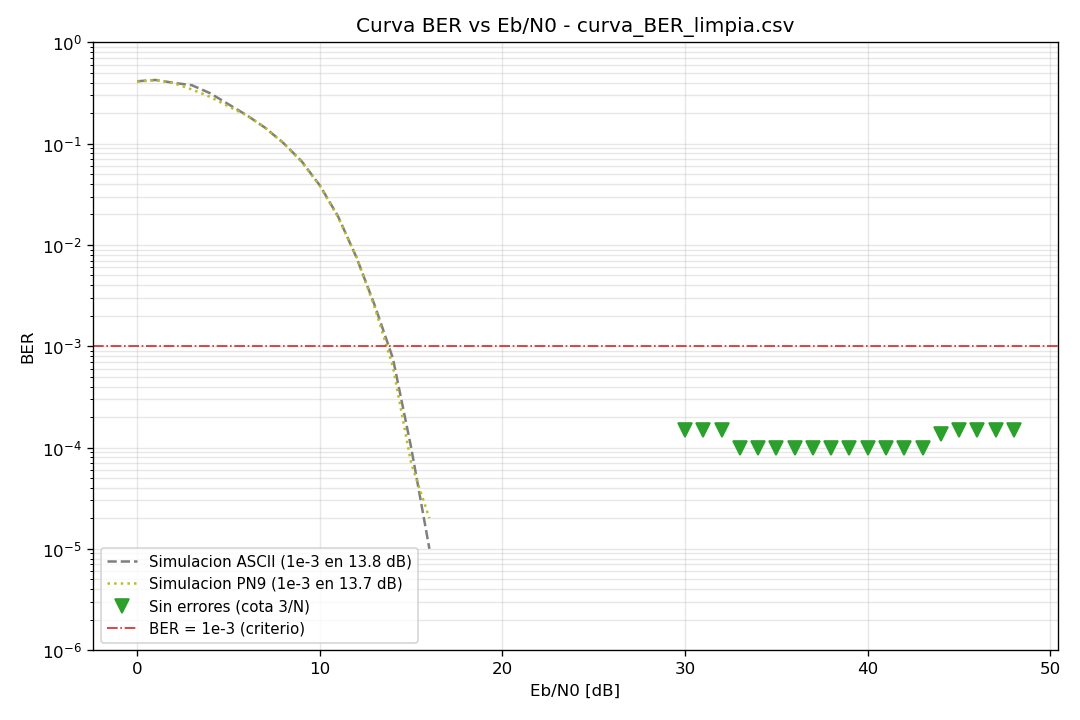
\includegraphics[width=\columnwidth]{limpia.png}
\caption{Condición limpia (barrido de 30 a 48~dB): $\text{BER} = 0$ en los 19 puntos. Los triángulos marcan la cota $3/N$; las curvas punteadas son la simulación de referencia.}
\label{fig:limpia}
\end{figure}

\begin{figure}[!t]
\centering
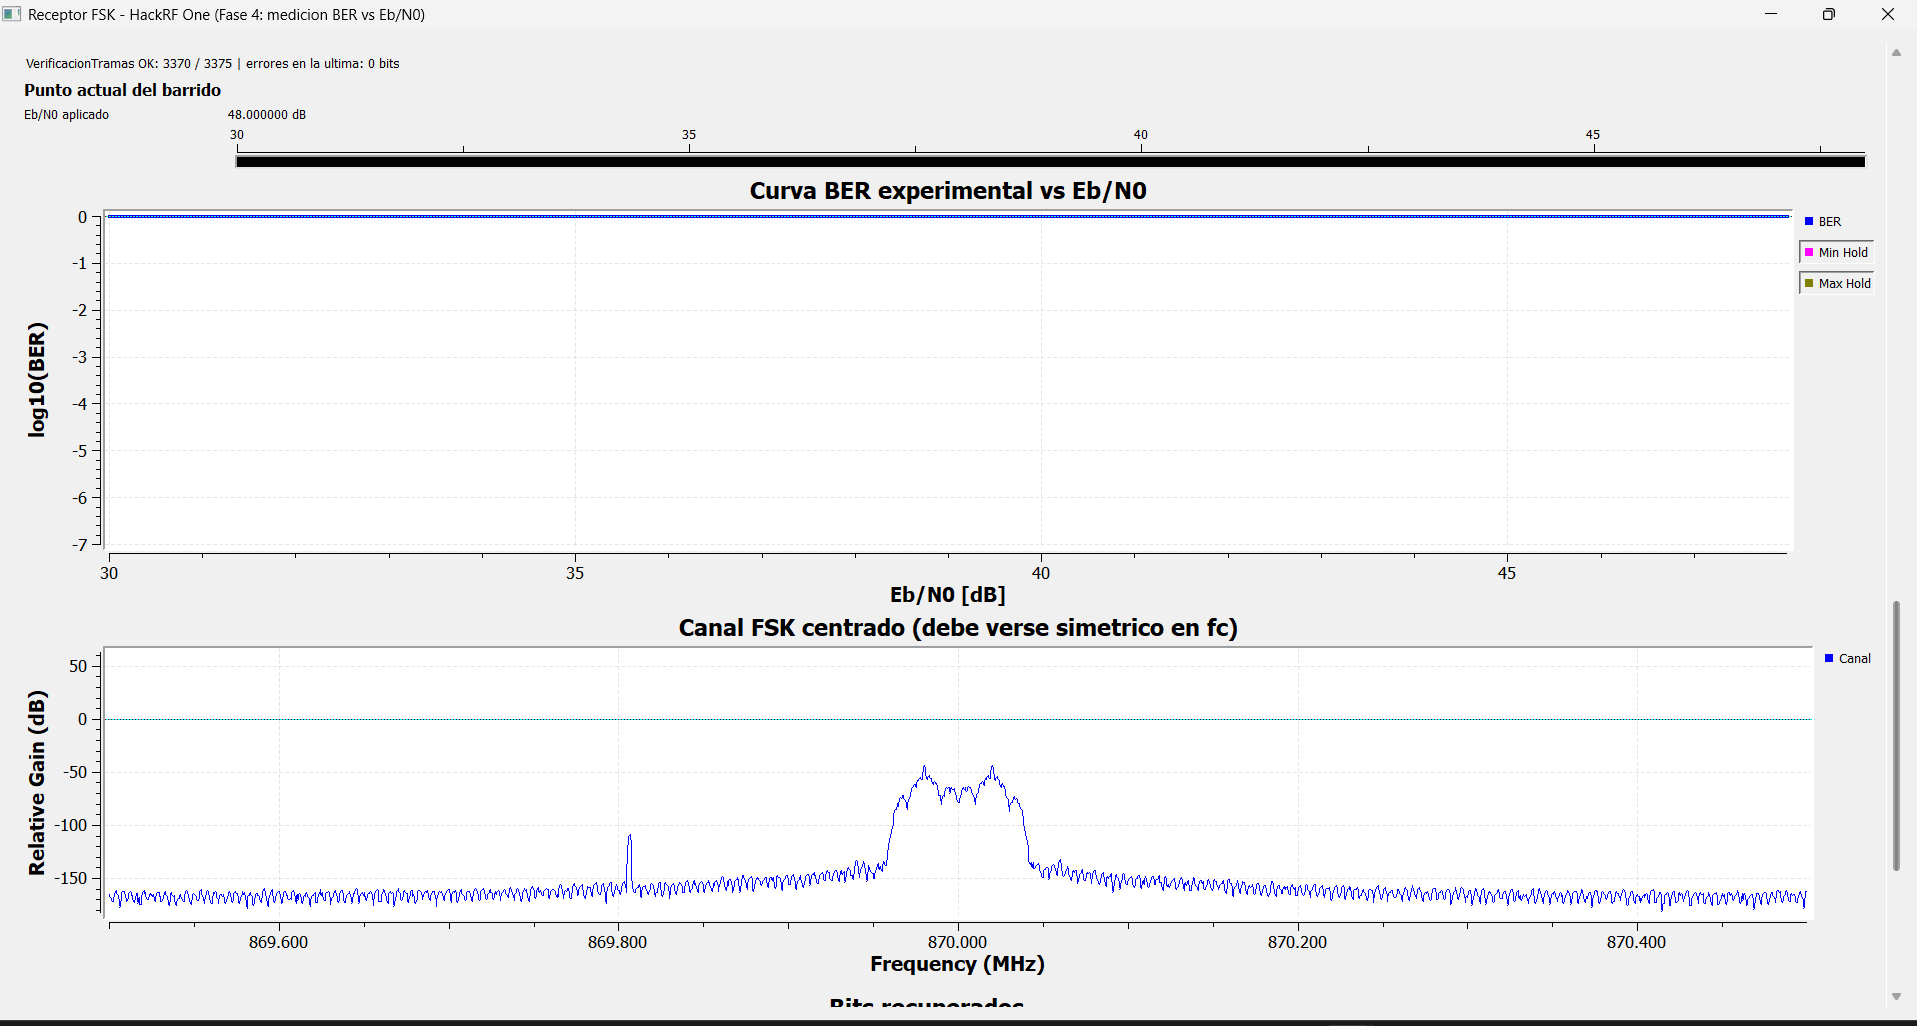
\includegraphics[width=\columnwidth]{limpia_gui.png}
\caption{GUI del receptor en condición limpia: verificación de tramas (3370/3375 correctas, 0 errores en la última), punto actual del barrido (48~dB) y canal FSK centrado y simétrico. La línea en 869.8~MHz es el pico de DC del HackRF, desplazado fuera del canal por \texttt{lo\_offset}.}
\label{fig:limpiagui}
\end{figure}

\subsection{Curvas BER vs. $E_b/N_0$}

Las Figs.~\ref{fig:medascii} y~\ref{fig:medpn9} muestran las dos mediciones válidas en GNU Radio, con la curva que se actualiza durante la ejecución, y la Fig.~\ref{fig:comp} las superpone a las curvas simuladas con el mismo receptor. La medición ASCII duró unos 12.5~min (cerca de 400\,000~bits por punto) y la PN9 unos 10~min (cerca de 300\,000~bits por punto). El Cuadro~\ref{tab:ber} resume los valores; los CSV originales, sin editar, se entregan en el repositorio.

\begin{figure*}[!t]
\centering
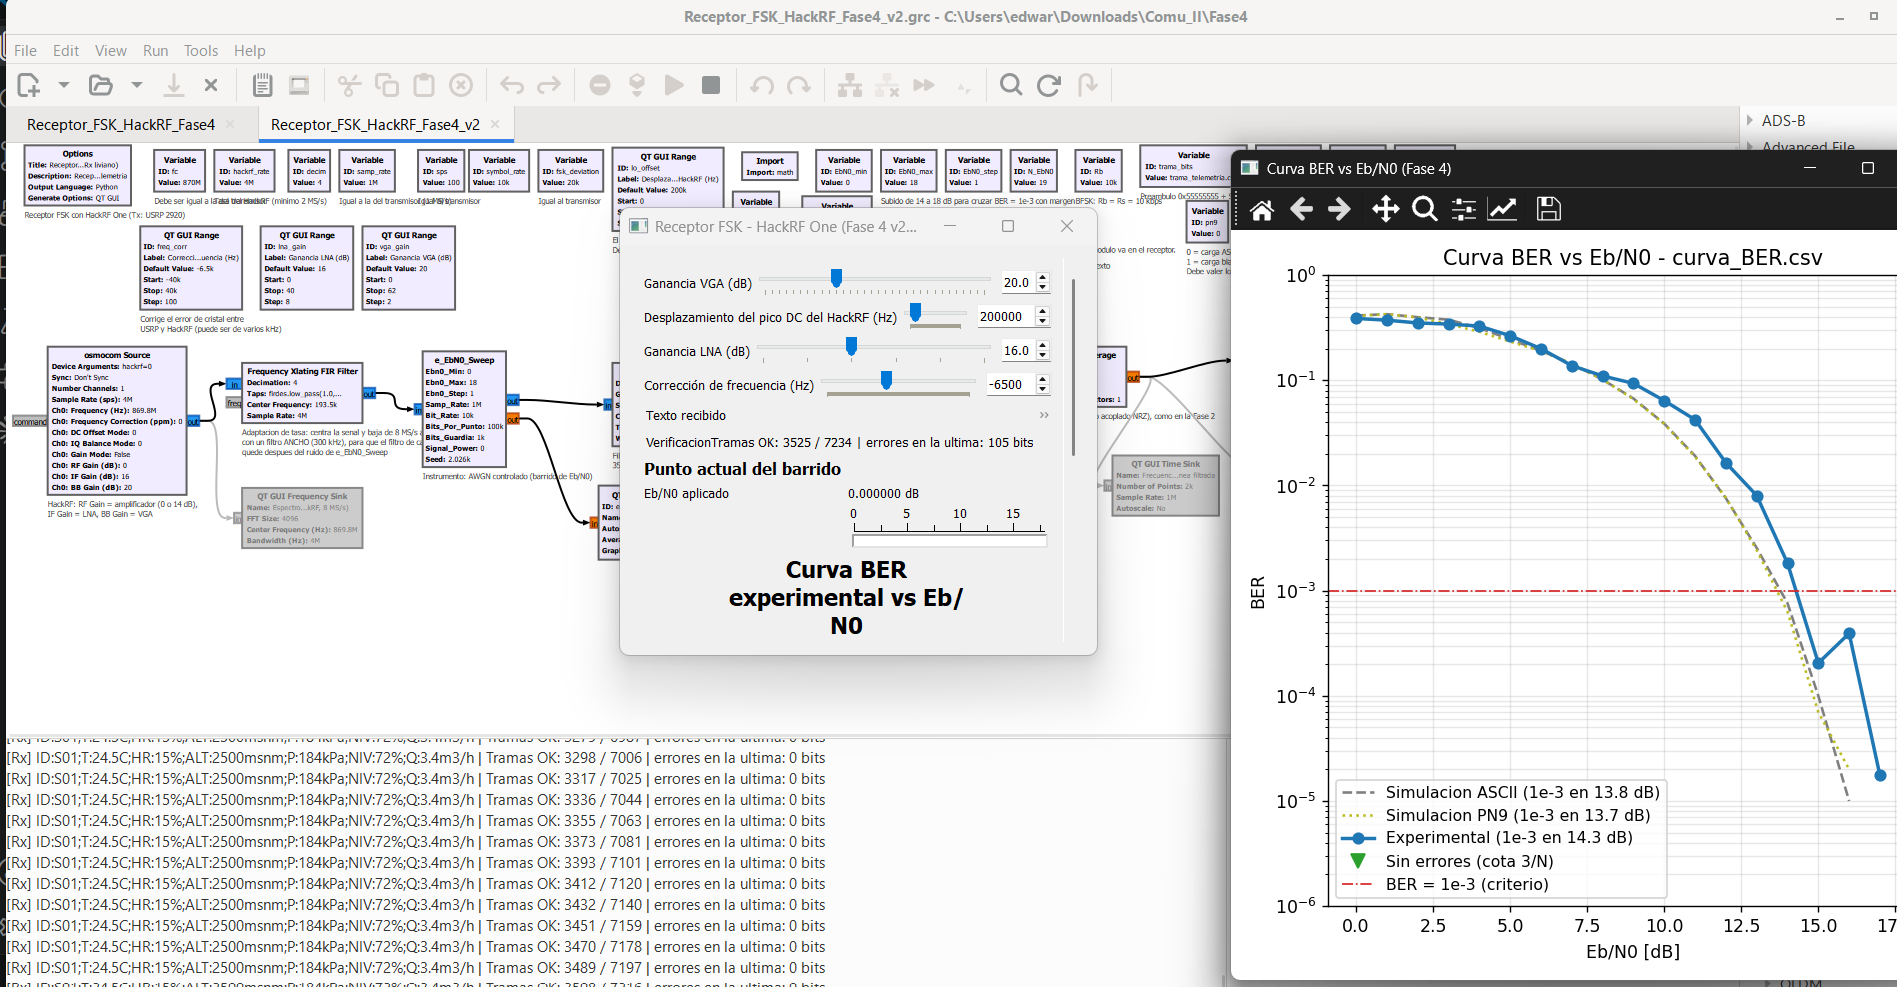
\includegraphics[width=0.85\textwidth]{med_ascii.png}
\caption{Medición ASCII (\texttt{pn9 = 0}) en GNU Radio: flujograma en ejecución, controles del receptor, verificación de texto en consola y curva BER medida frente a la simulada. $\text{BER} = 10^{-3}$ en 14.3~dB.}
\label{fig:medascii}
\end{figure*}

\begin{figure*}[!t]
\centering
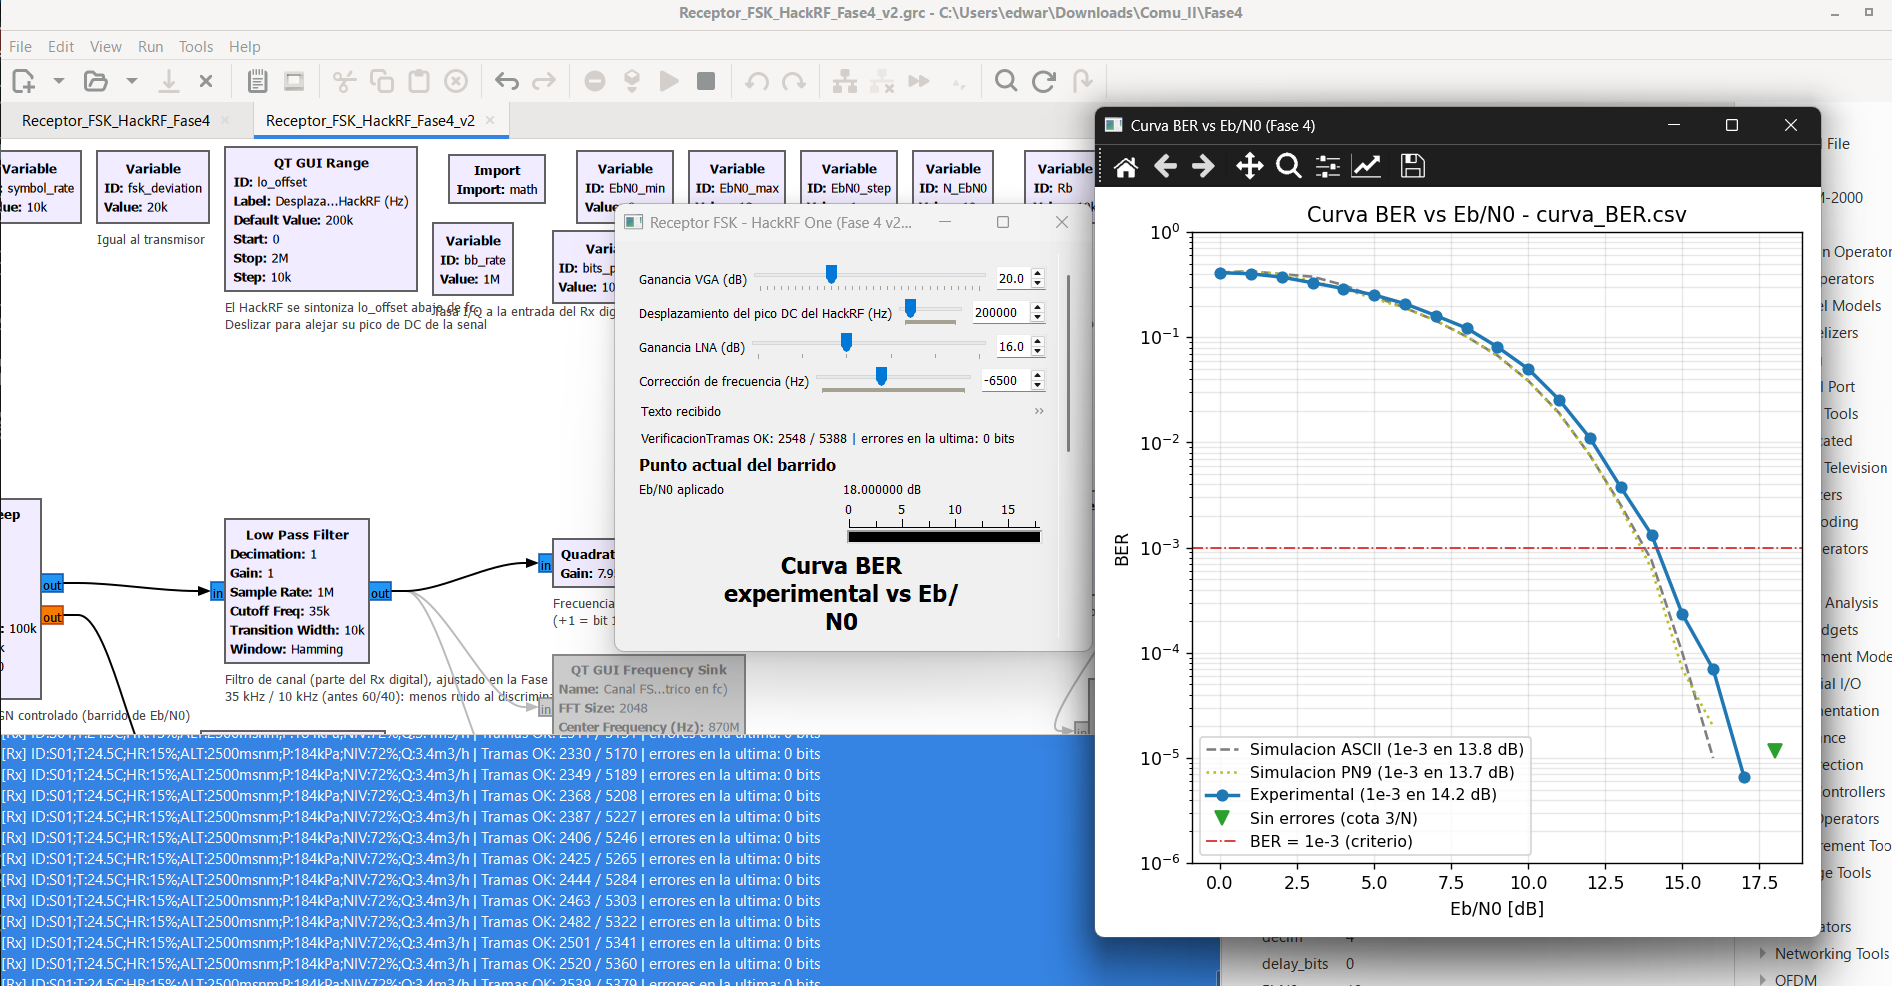
\includegraphics[width=0.85\textwidth]{med_pn9.png}
\caption{Medición PN9 (\texttt{pn9 = 1}) en GNU Radio. $\text{BER} = 10^{-3}$ en 14.2~dB.}
\label{fig:medpn9}
\end{figure*}

\begin{figure}[!t]
\centering
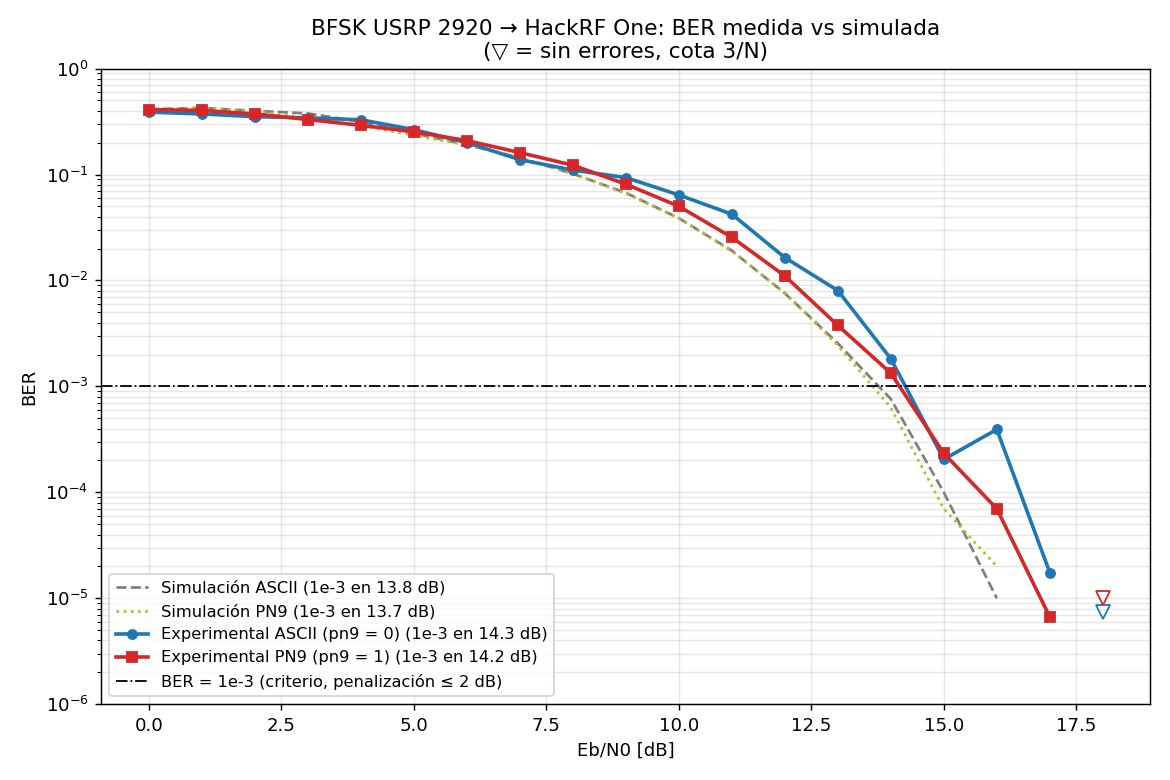
\includegraphics[width=\columnwidth]{comparacion.png}
\caption{BER medida frente a simulada para las dos variantes de la trama. La línea horizontal marca el punto de comparación, $\text{BER} = 10^{-3}$.}
\label{fig:comp}
\end{figure}

\begin{table}[!t]
\centering
\caption{BER medida en el enlace por aire.}
\label{tab:ber}
\begin{tabular}{ccc}
\toprule
$E_b/N_0$ (dB) & ASCII (\texttt{pn9 = 0}) & PN9 (\texttt{pn9 = 1}) \\
\midrule
0 & $3.9\times10^{-1}$ & $4.1\times10^{-1}$ \\
2 & $3.5\times10^{-1}$ & $3.7\times10^{-1}$ \\
4 & $3.3\times10^{-1}$ & $2.9\times10^{-1}$ \\
6 & $2.0\times10^{-1}$ & $2.1\times10^{-1}$ \\
8 & $1.1\times10^{-1}$ & $1.2\times10^{-1}$ \\
10 & $6.4\times10^{-2}$ & $5.0\times10^{-2}$ \\
11 & $4.2\times10^{-2}$ & $2.6\times10^{-2}$ \\
12 & $1.6\times10^{-2}$ & $1.1\times10^{-2}$ \\
13 & $8.0\times10^{-3}$ & $3.8\times10^{-3}$ \\
14 & $1.8\times10^{-3}$ & $1.3\times10^{-3}$ \\
15 & $2.1\times10^{-4}$ & $2.3\times10^{-4}$ \\
16 & $3.9\times10^{-4}$ & $7.0\times10^{-5}$ \\
17 & $1.8\times10^{-5}$ & $6.7\times10^{-6}$ \\
18 & 0 & 0 \\
\bottomrule
\end{tabular}
\end{table}

El Cuadro~\ref{tab:conf} aplica el criterio de la guía. El $E_b/N_0$ que da $\text{BER} = 10^{-3}$ se obtuvo interpolando en escala logarítmica entre 14 y 15~dB. En las dos variantes la penalización respecto a la simulación es de unos 0.5~dB, por lo que la medición es \textbf{conforme}.

\begin{table}[!t]
\centering
\caption{Comparación en $\text{BER} = 10^{-3}$ (criterio: penalización $\leq 2$~dB).}
\label{tab:conf}
\begin{tabular}{lcccc}
\toprule
Trama & Simulación & Medida & Penalización & Veredicto \\
\midrule
ASCII & 13.8~dB & 14.3~dB & 0.5~dB & Conforme \\
PN9 & 13.7~dB & 14.2~dB & 0.5~dB & Conforme \\
\bottomrule
\end{tabular}
\end{table}

\section{Análisis}

\subsection{Comportamiento de la BER}

Entre 0 y 5~dB la BER es de 0.3 a 0.4: el discriminador está por debajo de su umbral y el ruido domina la frecuencia instantánea. A partir de unos 8~dB la curva cae cada vez más rápido, como corresponde a una detección no coherente, y entre 12 y 15~dB baja casi una década por cada dB. Por encima de 17~dB no se observaron errores.

La referencia teórica de BFSK no coherente con detector óptimo de energía es~\cite{proakis}
\begin{equation}
P_b = \tfrac{1}{2}\, e^{-E_b/2N_0},
\end{equation}
que da $\text{BER} = 10^{-3}$ en 10.9~dB. El receptor del proyecto queda unos 3~dB por detrás, tanto en simulación como en hardware. Esa diferencia es propia del diseño y no del enlace: un discriminador seguido de un integrador no es el detector óptimo, y con $h = 4$ el filtro de canal debe dejar pasar unos 70~kHz para contener los dos tonos, mucho más que los $R_b = 10$~kHz que necesitaría un detector de energía por tono. Lo que se valida en esta fase es la penalización del \emph{hardware} respecto al mismo receptor simulado, que es de solo 0.5~dB.

Las posibles causas de esos 0.5~dB son:
\begin{itemize}
\item \textbf{Error de frecuencia residual.} \texttt{freq\_corr} se ajusta a mano con pasos de 100~Hz y los cristales derivan con la temperatura. En el banco de pruebas, un error de 2 a 5~kHz producía una penalización de unos 0.5~dB.
\item \textbf{Ruido propio del enlace.} \texttt{e\_EbN0\_Sweep} calcula el ruido a partir de la potencia total recibida $P_s$, que ya incluye el ruido térmico del HackRF y el del canal real. El $E_b/N_0$ efectivo es, por tanto, algo menor que el nominal.
\item \textbf{Imperfecciones del receptor de conversión directa}: residuos de DC y desbalance I/Q, cuantificación de 8~bits del HackRF y los bits descartados por realineos.
\end{itemize}

\subsection{ASCII frente a PN9}

Las dos curvas coinciden dentro de la variación estadística, pero la PN9 es más regular: es monótona y queda algo más cerca de la simulación entre 11 y 14~dB. La explicación está en el DC Blocker que sigue al demodulador. Ese bloque elimina el valor medio de la frecuencia instantánea, que debería deberse solo al error de frecuencia; pero con la carga ASCII la proporción de unos es 0.451, así que los datos tienen un valor medio propio de $2(0.451) - 1 \approx -0.10$ que el bloque también resta. El resultado es un desplazamiento del umbral de decisión, visible en el ojo de la Fig.~\ref{fig:ojo}, cuyos niveles quedan en aproximadamente $+1.2$ y $-0.8$ en lugar de $\pm 1$. Con la carga blanqueada la proporción de unos es 0.498 y el desplazamiento desaparece. Es la misma razón por la que los estándares de telemetría como 802.15.4g blanquean la carga~\cite{ieee154g}.

La anomalía de la curva ASCII en 16~dB ($3.9\times10^{-4}$, peor que en 15~dB) corresponde a pocos errores agrupados, compatibles con un episodio aislado de pérdida de muestras o una perturbación del entorno durante ese tramo; no aparece en la medición PN9.

\begin{figure}[!t]
\centering
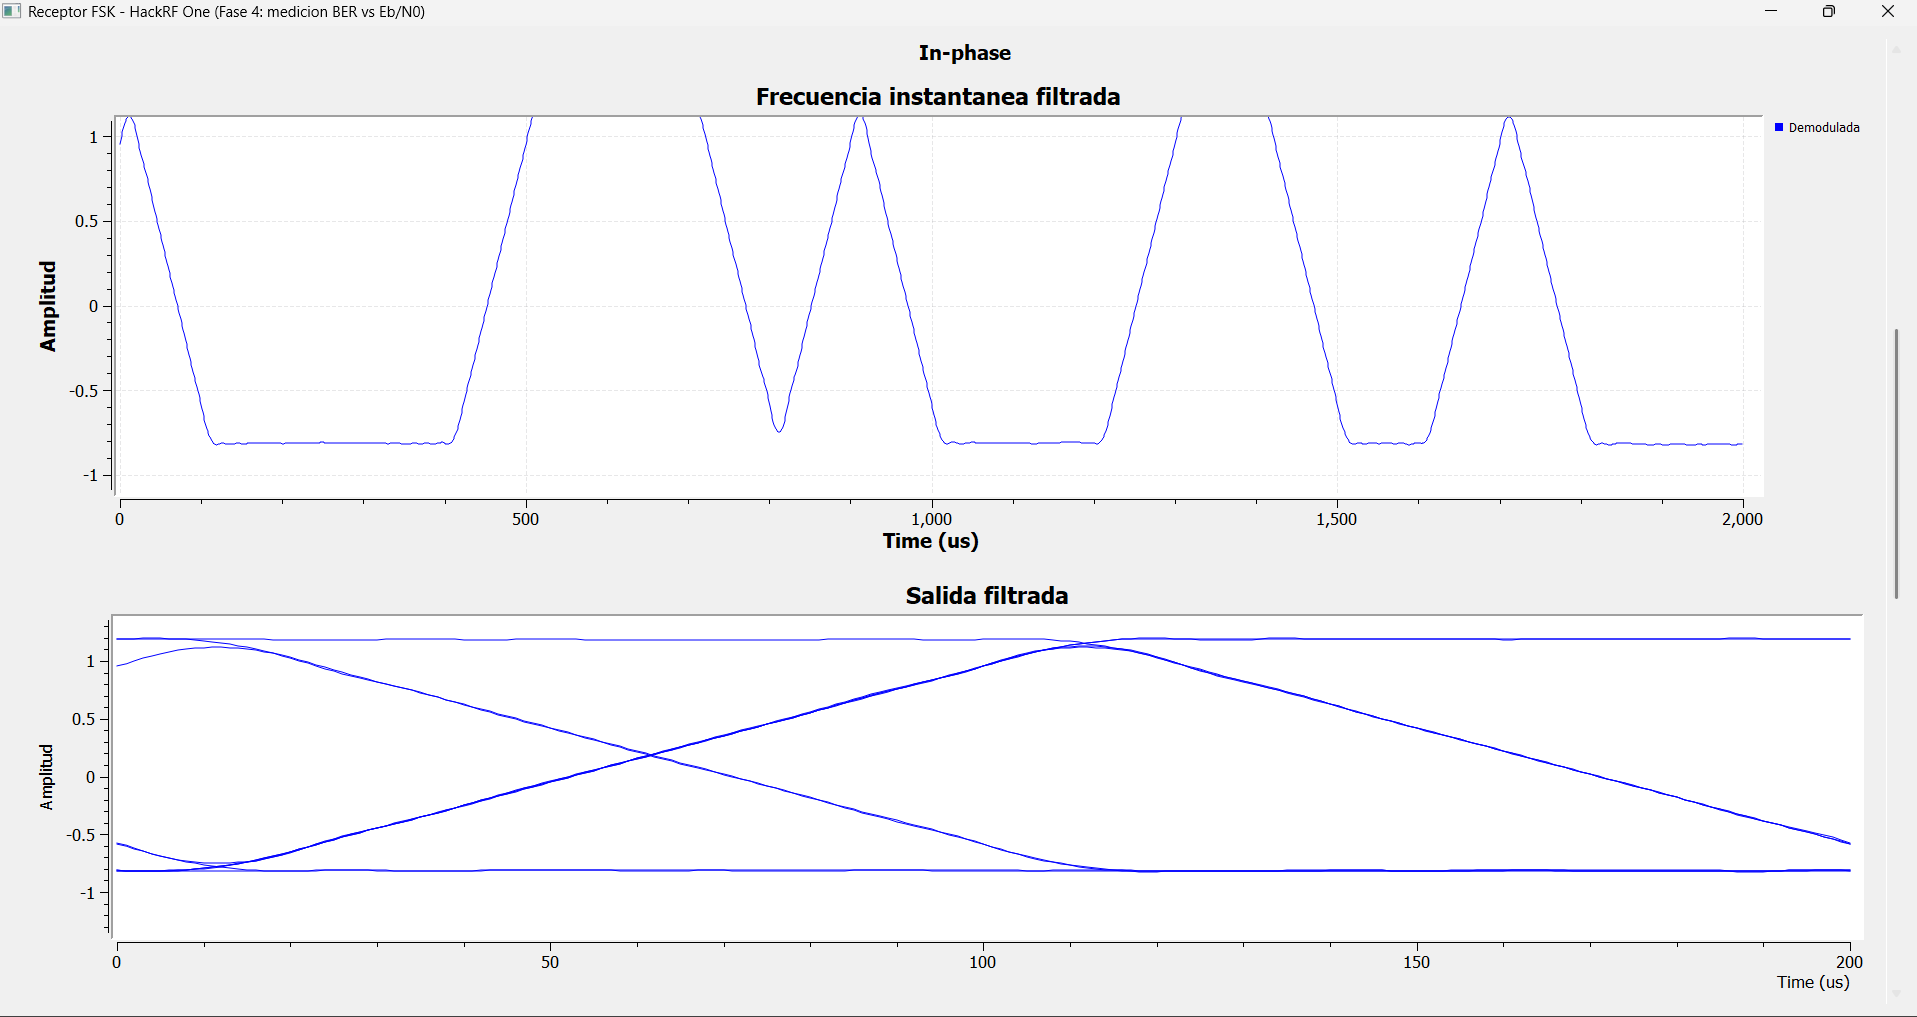
\includegraphics[width=\columnwidth]{ojo.png}
\caption{Frecuencia instantánea filtrada y diagrama de ojo a la salida del integrador durante el ajuste (carga ASCII, sin ruido añadido). El ojo está completamente abierto, pero sus niveles son asimétricos (aprox. $+1.2$ y $-0.8$) por el valor medio de los datos que elimina el DC Blocker.}
\label{fig:ojo}
\end{figure}

\subsection{SNR asociada al barrido}

La columna $E_b/N_0$ es la condición que aplica el barrido, no una medida de la SNR. La relación entre ambas se obtiene de~\eqref{eq:pn}: la SNR sobre todo el ancho de banda de la muestra es
\begin{equation}
\text{SNR}_{f_s} = \frac{E_b}{N_0} + 10\log_{10}\frac{R_b}{f_s} = \frac{E_b}{N_0} - 20~\text{dB},
\end{equation}
y la SNR dentro del canal útil, con un ancho de ruido de unos $B_{ch} \approx 70$~kHz (filtro de $\pm 35$~kHz), es
\begin{equation}
\text{SNR}_{ch} = \frac{E_b}{N_0} + 10\log_{10}\frac{R_b}{B_{ch}} \approx \frac{E_b}{N_0} - 8.5~\text{dB}.
\end{equation}
En el punto de comparación ($E_b/N_0 \approx 14.2$~dB) la SNR en el canal es de unos 5.7~dB, mientras que sobre 1~MHz es negativa ($-5.8$~dB). Esto explica por qué el filtro de canal es crítico: sin él el discriminador trabajaría con una SNR 11.5~dB peor y caería en el efecto umbral, como ya se observó en la simulación de la Fase~2.

Estos valores son calculados a partir del ruido añadido. La SNR real es algo menor, porque $P_s$ incluye el ruido del propio enlace por aire; esa diferencia es una de las causas de la penalización de 0.5~dB.

\subsection{Dispersión I/Q}

FSK tiene envolvente constante, por lo que la señal I/Q ideal recorre un círculo de radio $A$ y la dispersión se manifiesta como un engrosamiento del anillo. Sin ruido añadido, la Fig.~\ref{fig:iq}b muestra un anillo delgado y circular, de radio cercano a 0.042 en unidades del ADC: la dispersión que introduce el enlace por aire es pequeña, coherente con la BER nula en condición limpia. La Fig.~\ref{fig:iq}a muestra en cambio la dispersión que producen las imperfecciones del hardware y no el ruido: con $\texttt{lo\_offset} = 0$ y ganancias altas (LNA 24~dB, VGA 62~dB), el desbalance I/Q y el DC del HackRF convierten el círculo en una elipse ancha. Corregir ese efecto con \texttt{lo\_offset} = 200~kHz y ganancias moderadas fue uno de los ajustes que permitió obtener la curva.

Con el ruido del barrido, la dispersión relativa esperada es $\sqrt{P_n/P_s}$. Antes del filtro de canal vale $\sqrt{100/(E_b/N_0)}$, es decir, entre 10 (0~dB) y 1.3 (18~dB): el anillo desaparece por completo en todo el rango del barrido. Después del filtro, el ruido se reduce en la relación $B_{ch}/f_s \approx 0.07$ y la dispersión relativa baja a unos 0.53 en 14~dB. En la constelación de decisión, la simulación de la Fase~2 con el mismo receptor dio dos nubes en $\pm 0.97$ con desviación de 0.02 sin ruido, y en $\pm 0.88$ con desviación de 0.20 a 12~dB, donde la BER ya es del orden de $10^{-2}$. Durante la medición en hardware las gráficas I-Q estaban deshabilitadas para evitar pérdidas de muestras, por lo que la dispersión I/Q no se midió en función de $E_b/N_0$; el análisis anterior es teórico y se apoya en las capturas del ajuste y en la simulación.

\begin{figure}[!t]
\centering
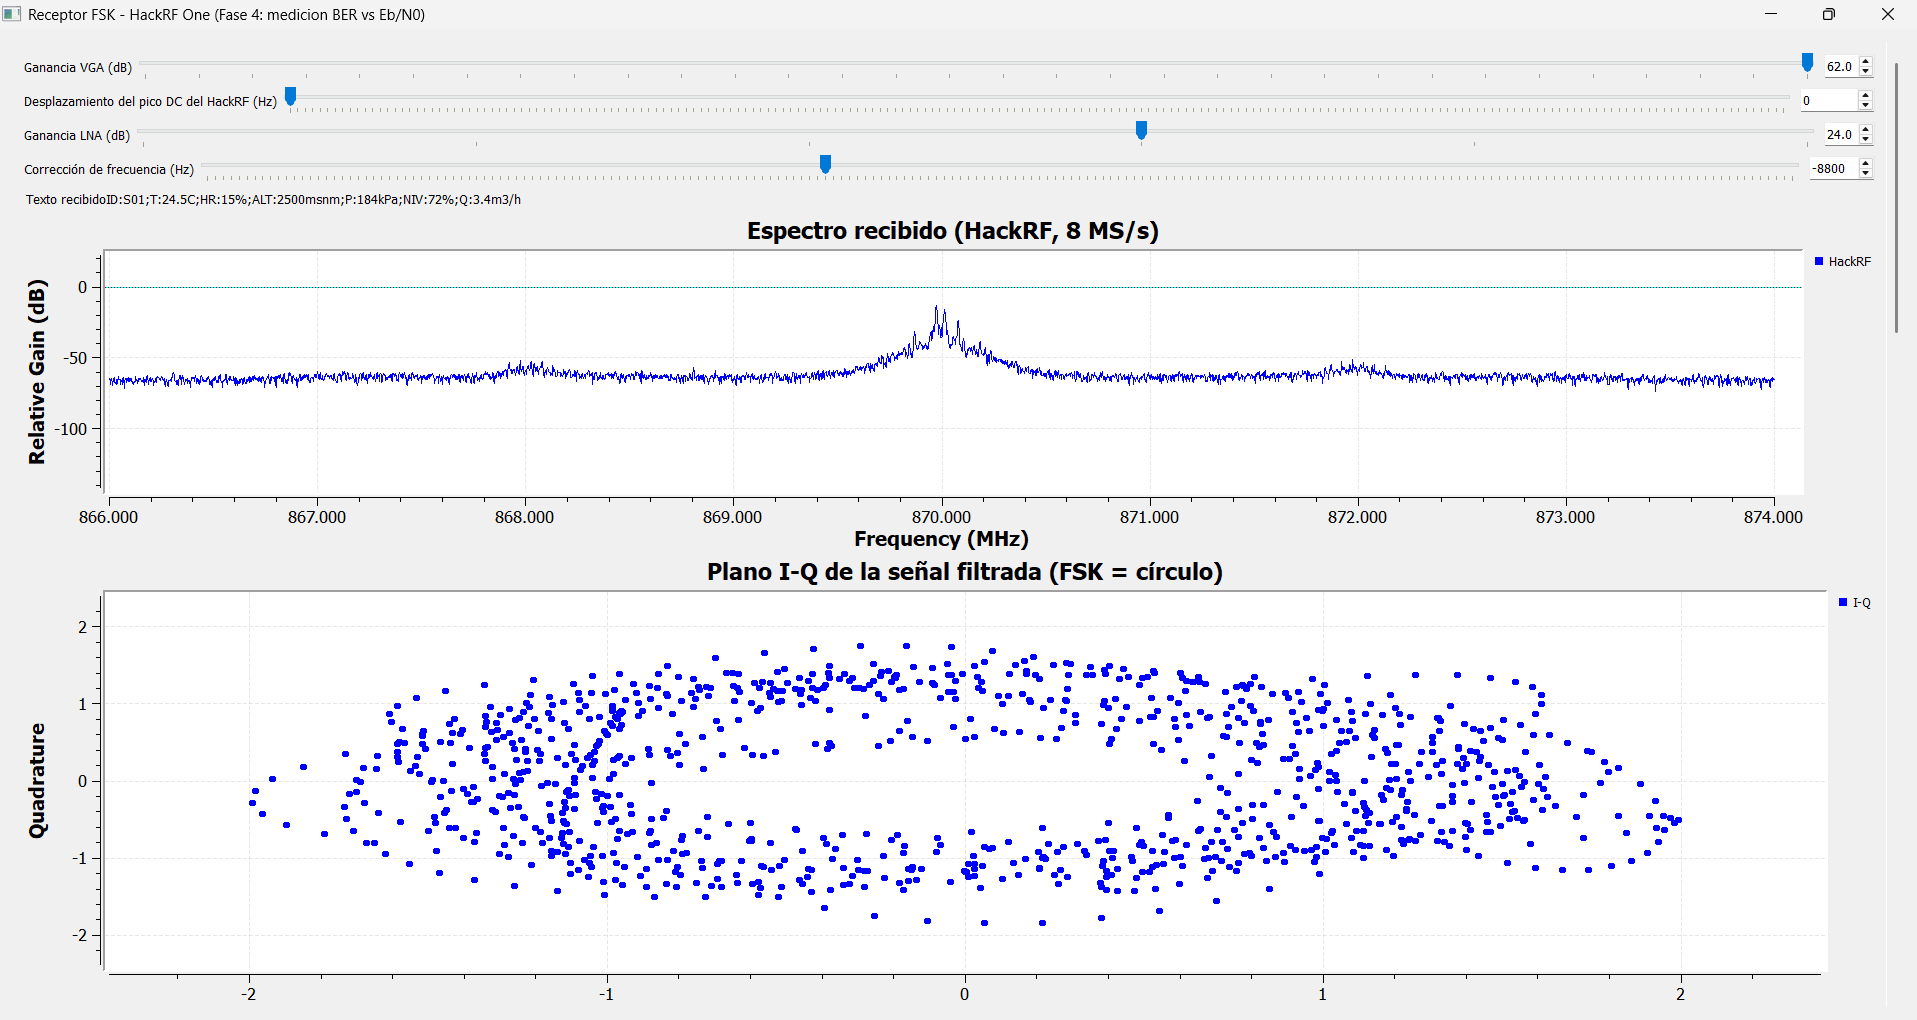
\includegraphics[width=\columnwidth]{iq_lo0.png}\\[2pt]
\small (a)\\[2pt]
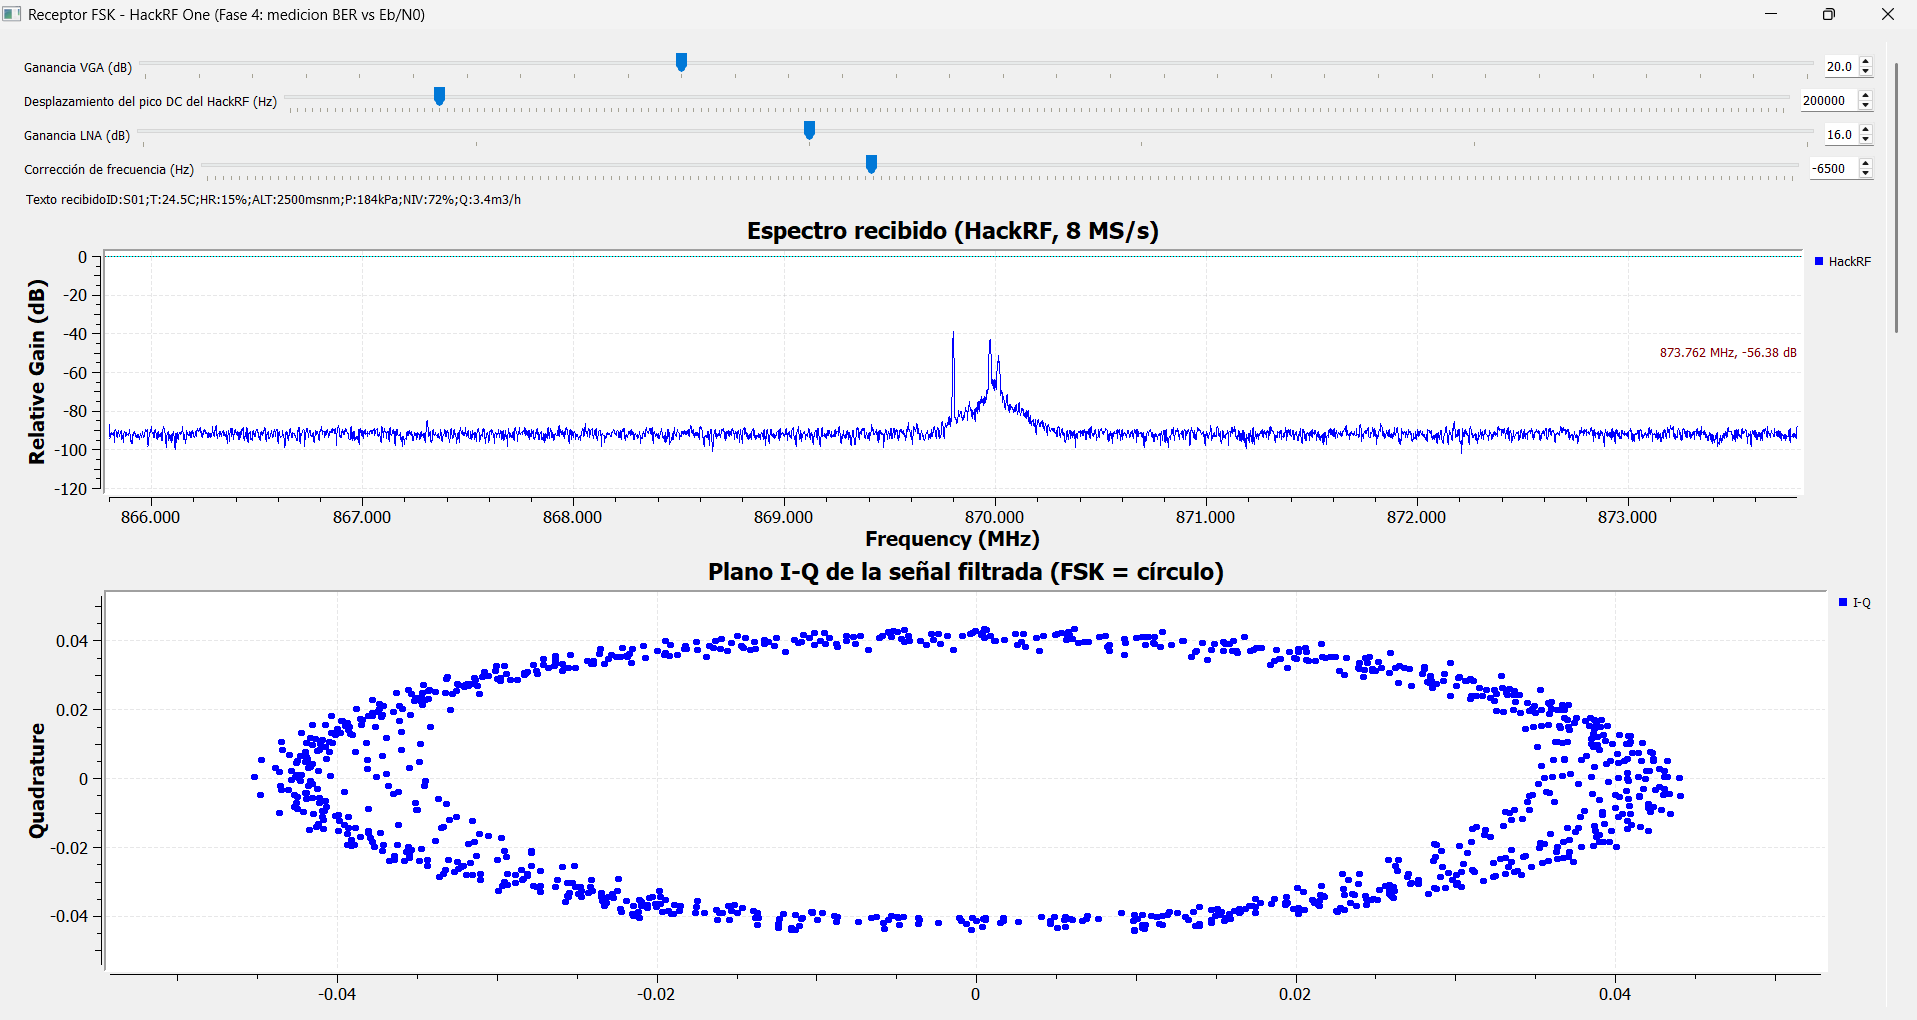
\includegraphics[width=\columnwidth]{iq_lo200k.png}\\[2pt]
\small (b)
\caption{Espectro recibido y plano I-Q de la señal filtrada durante el ajuste. (a) $\texttt{lo\_offset} = 0$, LNA 24~dB, VGA 62~dB: el pico de DC cae sobre la señal y el desbalance I/Q deforma el anillo en una elipse dispersa. (b) $\texttt{lo\_offset} = 200$~kHz, LNA 16~dB, VGA 20~dB: anillo delgado y circular; el texto llega completo en ambos casos.}
\label{fig:iq}
\end{figure}

\section{Problemas encontrados}

El Cuadro~\ref{tab:err} reúne los problemas de la integración y de la medición, junto con su solución. Los cambios en el código del kit se hicieron solo en la copia de trabajo y están marcados con el comentario \texttt{\# Ajuste Fase 4}.

\begin{table*}[!t]
\centering
\caption{Problemas encontrados durante la integración y la medición.}
\label{tab:err}
\begin{tabular}{>{\raggedright}p{4.2cm}>{\raggedright}p{6.2cm}p{6.2cm}}
\toprule
Problema & Causa & Solución \\
\midrule
La plantilla del kit no compilaba en GNU Radio 3.10.12. & \texttt{e\_BER\_Curve} heredaba de \texttt{gr.sync\_decimator}, una clase C++ que no sirve para bloques en Python. & Herencia de \texttt{gr.decim\_block}, con la misma lógica. \\
Error al validar el bloque que guarda el CSV. & Usaba \texttt{\_\_file\_\_}, que GRC no define al validar. & Usar el directorio de trabajo si \texttt{\_\_file\_\_} no existe. \\
Error de conexión ``IO size 60 vs 76''. & GRC dimensiona los puertos vectoriales con los valores por defecto del código (15 puntos). & Valor por defecto de 19 puntos, igual al barrido. \\
BER de 0.3--0.4 con el texto llegando perfecto. & Overflows del HackRF al abrir la GUI: se pierden muestras y el flujo salta bits; la referencia solo corregía saltos de $\pm 3$~bits. & Realineación global en \texttt{e\_Ref\_Alineada}. \\
Piso falso de BER ($10^{-2}$ a $6\times10^{-2}$) en el primer barrido. & Tras cada realineo se comparaban 1000 a 2000~bits con la referencia desalineada. & Etiqueta \texttt{realineo} y descarte de 8000~bits antes y 1000 después; receptor liviano (gráficas pesadas deshabilitadas, HackRF a 4~MS/s). \\
Medición PN9 invalidada (más de 15 realineos). & Uso del portátil del receptor (captura de pantalla) a mitad de la corrida. & Repetir sin tocar el portátil; capturas solo al final. \\
El bloque del CSV dejaba de guardar. & Otro programa tenía abierto \texttt{curva\_BER.csv} y Windows no permitía reemplazarlo. & Reintento en el siguiente guardado. \\
La QT GUI Vector Sink no dibujaba la curva. & La gráfica se quedaba en 0 aunque el CSV era correcto; no se aisló la causa. & Visor externo en Python que lee el CSV y superpone la simulación (Figs.~\ref{fig:medascii} y~\ref{fig:medpn9}). \\
Plano I-Q elíptico. & Pico de DC y desbalance I/Q del HackRF dentro del canal. & $\texttt{lo\_offset} = 200$~kHz. \\
\bottomrule
\end{tabular}
\end{table*}

\begin{figure}[!t]
\centering
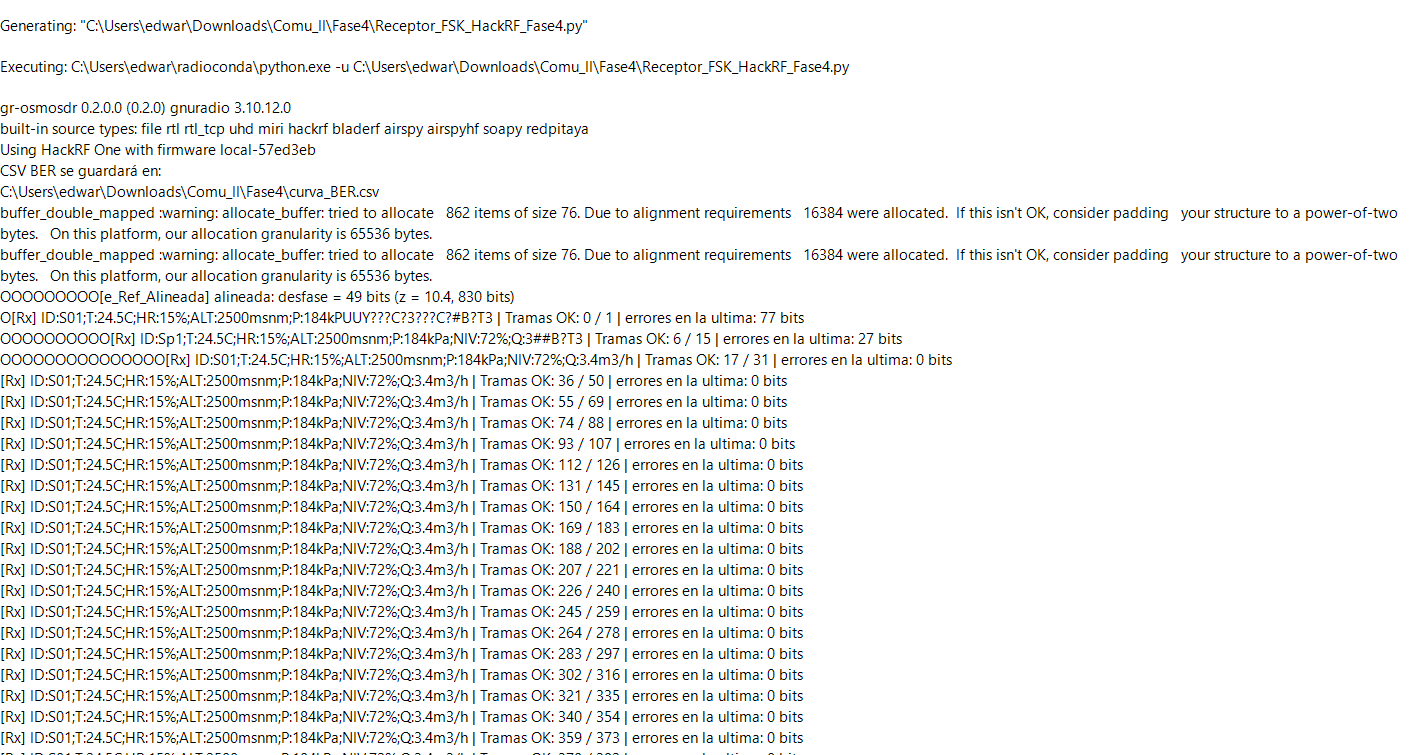
\includegraphics[width=\columnwidth]{consola.png}
\caption{Consola del receptor al arrancar: overflows del HackRF (``O''), alineación de la referencia (desfase de 49~bits, $z = 10.4$) y verificación de las tramas de texto, que pasan a llegar sin errores.}
\label{fig:consola}
\end{figure}

\section{Conclusiones}

Se integró el módulo común de instrumentación BER en una copia del receptor del proyecto, insertando el ruido controlado después de la adaptación de tasa del HackRF (1~MS/s) y antes del filtro de canal, y se midió la curva BER vs. $E_b/N_0$ del enlace BFSK real entre un USRP 2920 y un HackRF One a 870~MHz con los parámetros de diseño de la aplicación: $R_b = 10$~kb/s, $\Delta f = 20$~kHz y $sps = 100$.

La primera medición mostró que el receptor de la Fase~3, suficiente para ver los bits sin ruido, tenía un desempeño pobre: el filtro de canal era demasiado ancho y el muestreo fijo no seguía la deriva de reloj entre radios. Con un filtro de canal de 35~kHz, un integrador como filtro acoplado y un sincronizador de símbolo de Gardner, el receptor alcanzó en hardware $\text{BER} = 10^{-3}$ en 14.3~dB con la carga ASCII y en 14.2~dB con la carga PN9, apenas 0.5~dB por detrás de la simulación y dentro del criterio de 2~dB. En condición limpia la BER fue nula.

Las principales limitaciones observadas no vinieron del canal, sino del sistema de recepción: la pérdida de muestras del HackRF cuando el portátil está ocupado, que obligó a alinear la referencia automáticamente y a no usar el equipo durante la medición; el error de frecuencia entre cristales, que se corrige a mano; y el DC y el desbalance I/Q del receptor de conversión directa. Además, el receptor diseñado queda unos 3~dB por detrás del detector no coherente óptimo, el costo de usar un discriminador con un índice de modulación alto. Como mejoras quedan la corrección automática de frecuencia, un detector de energía por tono y la medición conducida con cable y atenuadores, que eliminaría la incertidumbre del canal por aire.

\begin{thebibliography}{9}

\bibitem{guia1} Universidad Industrial de Santander, ``Proyecto Final de Comunicaciones II -- Fase 2: Modelado y Simulación (Guía 1)'', Guía de laboratorio.

\bibitem{guia2} Universidad Industrial de Santander, ``Proyecto Final de Comunicaciones II -- Diseño del Sistema Tx--Canal--Rx en GNU Radio (Guía 2)'', Guía de laboratorio.

\bibitem{guia3} O. Tíjaro y R. Zamora, ``Proyecto Final de Comunicaciones II -- Fase 3: Configuración inicial de HackRF One y USRP en GNU Radio (Guía 3)'', Universidad Industrial de Santander.

\bibitem{guia4} O. Tíjaro y R. Zamora, ``Proyecto Final de Comunicaciones II -- Fase 4: Validación final, ajuste y comparación experimental (Guía 4)'', Universidad Industrial de Santander.

\bibitem{guia4a} O. Tíjaro y R. Zamora, ``Proyecto Final de Comunicaciones II -- Fase 4: Integración del módulo BER y extracción automática de métricas en CSV (Guía 4A)'', Universidad Industrial de Santander.

\bibitem{proakis} J. G. Proakis y M. Salehi, \textit{Digital Communications}, 5th ed., McGraw-Hill, 2008.

\bibitem{symsync} GNU Radio Project, ``Symbol Sync'', disponible en: \url{https://wiki.gnuradio.org/index.php/Symbol_Sync}.

\bibitem{ieee154g} IEEE, ``IEEE Std 802.15.4g-2012: Physical Layer Specifications for Low-Data-Rate, Wireless, Smart Metering Utility Networks'', 2012.

\end{thebibliography}

\end{document}
